\documentclass[12pt, a4paper]{article}

\usepackage[T1, T2A]{fontenc}
\usepackage[utf8]{inputenc}
\usepackage[english, russian]{babel}
\usepackage{amsmath, amssymb}
\usepackage[left=3cm, right=1.5cm, top=2cm, bottom=2cm]{geometry}
\usepackage[displaymath]{lineno}
\usepackage[space]{cite}
\usepackage{xcolor, graphicx}

\usepackage{amsmath}
% Отключаем привязку нумерации к секциям в основном тексте
\counterwithout{equation}{section}
% Настройка для приложений
\usepackage{etoolbox}
\appto\appendix{%
	\renewcommand{\theequation}{П\arabic{equation}}%
	\setcounter{equation}{0}%
}


\renewcommand{\vec}{\mathbf}
\linenumbers
\linespread{2}

\def \eps {\varepsilon}
\def \w {\omega}
\def \ph {\varphi}
\def \kp { \varkappa}
\def \ex { \operatorname{ex}}
\def \out { \operatorname{out}}

\newcommand{\rd}[1]{\color{red} #1 \color{black}}

\newcommand{\op}[1]{\operatorname {#1}}

\newcommand{\dt}[1]{\frac{\partial {#1}}{\partial t}}
\newcommand{\dx}[1]{\frac{\partial {#1}}{\partial x}}
\newcommand{\dn}[1]{\left.\frac{\partial #1}{\partial \vec{n}}\right|_{ S}}
\newcommand{\dr}[1]{\left.\frac{\partial #1}{\partial r}\right|_{ r = a}}
\newcommand{\sumexp}[1]{\frac{{#1} e^{i \w t} + {#1}^* e^{-i \w t}}{2}}
\newcommand{\sumexptwo}[1]{\frac{{#1} e^{2 i \w t} + {#1}^* e^{-2 i \w t}}{2}}
\newcommand{\dtau}[1]{\frac{\partial {#1}}{\partial \tau}}
\begin{document}
\thispagestyle{empty}

 \ Контактные данные автора, ответственного за связь с редакцией\\
Павличенко Иван Александрович\\
Нижегородский госуниверситет им. Н.\,И. Лобачевского, 603022, г. Нижний Новгород, пр.Гагарина, 23\\
контактный телефон {+7 831 465-60-35}\\
e-mail: pavlichenko@rf.unn.ru 

\newpage
\setcounter{page}{1}

УДК 533.98{:}533.9...12
\begin{center}
\large\bf ВОЗБУЖДЕНИЕ ДВОЙНЫХ ПЛАЗМОННЫХ\\ РЕЗОНАНСОВ В СФЕРИЧЕСКОЙ МЕТАЛЛИЧЕСКОЙ\\НАНОЧАСТИЦЕ
\end{center}

И.\,А. Павличенко$^{1}$, М.\,Р. Удалов$^{1}$

$^1$ Нижегородский госуниверситет им. Н.\,И. Лобачевского, г. Нижний Новгород;\\

В работе теоретически исследуется нелинейное взаимодействие сферической металлической наночастицы с внешним электромагнитным полем с учетом пространственной дисперсии и возбуждения второй гармоники.
Впервые рассмотрен случай двойных плазмонных резонансов, когда одновременно частоты основной и удвоенной гармоник поля совпадают с частотой Ми и частотой одного из объемных плазмонов наночастицы, соответственно.
На основе гидродинамической модели рассчитана средняя мощность потерь энергии.
Расчеты показали, что максимальное значение мощности потерь 
чувствительно к изменению величины диэлектрической проницаемости среды, окружающей наночастицу, и заметным образом возрастает при выполнении условий возбуждения двойных резонансов.
Полученные результаты показывают возможность использования данного эффекта для управления нелинейными оптическими свойствами наноструктур и нужд оптической диагностики.


\newpage

{\large\bf TITLE IN ENGLISH}

I.\,I. Ivanov, S.\,S. Safina, and P.\,P. Petrov

The abstract in English should be translated from the abstract in Russian.\\

Здесь желательно привести перевод часто используемых в статье специальных терминов на английский язык:\\
захваченные частицы --- trapped particles

\newpage

\section*{В\,В\,Е\,Д\,Е\,Н\,И\,Е}

Металлические наноструктуры привлекают к себе большое внимание благодаря своим уникальным характеристикам, связанным с возможностью возбуждения в них плазмонных резонансов на частоте падающего на наночастицу электромагнитного излучения.
Основной интерес к таким плазмонным наноструктурам обусловлен их способностью локализовать электромагнитные поля на нанометровых масштабах, существенно меньших дифракционного предела, что позволяет контролировать свойства света в размерах, намного меньших его длины волны \cite{Mai2007, Gram2010}.
Благодаря плазмонным резонансам в наноструктурах происходит существенное увеличение локальной плотности энергии поля, что приводит к возможности проявления в них различного рода нелинейных эффектов, таких как, например, многофотонная люминесценция \cite{Cas2011,biagioni2012,chen2021, ko2011}, четырехволновое смешивание \cite{danckwerts2007, harutyunyan2012, paspalakis2014, singh2016} и генерация гармоник оптического излучения \cite{drobyh2020, smirnova2014, TorresTorres2010}.
В частности, явление генерации второй гармоники в наноструктурах  (возможность возникновения которого в ограниченных металлических объектах была впервые обнаружена экспериментально и объяснена теоретически в работах \cite{franken1961, Bloembergen1962}) является в настоящее время основой для широкого круга практических применений, включающего диагностику наноструктур и оптических сред (см., например, \cite{butet2015, Butet2012}).

Важным фактором, благодаря которому наноструктуры и основанные на них метаматериалы могут служить эффективным инструментом для генерации второй гармоники, является возможность резонансного усиления поля не только основной гармоники оптического излучения, но и его второй гармоники при совпадении удвоенной частоты с собственной частотой другой плазмонной модой наноструктуры. 
К настоящему моменту явление двойного плазмонного резонанса исследовалось фактически только для наноструктур обеспечивающих одновременное возбуждение двух различных поверхностных плазмонов наночастицы на основной и удвоенной гармониках падающего излучения [ссылки].
Однако в общем случае в наноструктуре, помимо поверхностных плазмонов могут существовать и объемные плазмоны \cite{Elibol2022,Gildenburg2016,Ruppin1975,Gildenburg1965} -- моды коллективных электронных колебаний, представляющие собой стоячие плазменные (Ленгмюровские) волны и возникающие из-за пространственной дисперсии. 
%(нелокальности поляризуемости плазмы).
 Объемные плазмоны, как известно, могут сильно проявлять себя в случае, когда источник возбуждения коллективных электронных колебаний находится внутри наночастицы и характеризуется неоднородным распределением поля, что, например, имеет место в задачах спектроскопии характеристических потерь энергии электронами (англ. Electron Energy Loss Spectroscopy) при прохождении  пучка заряженных частиц через объем наноструктуры
\cite{Gildenburg2016, Kryshtal2025}. 
Подобная ситуация может возникнуть и в задачах генерации второй гармоники, когда обусловленные нелинейностью токи второй гармоники, возбуждаемые при резонансе поверхностного плазмона на основной частоте колебаний, могут возбуждать объемные плазмонные колебания в наночастице. Данный эффект может иметь место, например, в случае наноструктуры простейшей формы, металлической сферической наночастицы, однако к настоящему моменту двойные плазмонные резонансы типа <<поверхностный плазмон -- объемный плазмон>> фактически не были исследованы и являются предметом исследования данной работы.

В данной работе на основании гидродинамического подхода \cite{Haas2011, Boardman1982, Manfredi2021} исследуются нелинейные эффекты, обусловленные возникновением резонансов объемных плазмонов на удвоенной частоте в условиях, когда частота основной гармоники наночастицы также испытывает резонанс и совпадает с частотой дипольного поверхностного плазмона наночастицы (хорошо известный резонанс Ми). Работа организована следующим образом: вначале на основе уравнений гидродинамики с использованием метода последовательных приближений сформулированы краевые задачи, описывающие в квазистатическом приближении пространственное распределение поля и плотности заряда на основной и удвоенной гармониках внешнего поля в малой металлической наночастице произвольной формы. Далее описано решение этих задач применительно к случаю сферической наночастицы, и исследованы условия отвечающие условию возбуждения в наночастицах двойных резонансов типа поверхностный плазмон – объемный плазмон. В последующем разделе приведены результаты расчетов, иллюстрирующие влияние исследуемых резонансов на частотные зависимости сечения поглощения сферических наночастиц и сформулированы основные результаты работы.


\section{ПОСТАНОВКА ЗАДАЧИ}

{Рассмотрим металлическую наночастицу }произвольной формы, находящуюся в заданном внешнем поле падающей электромагнитной волны, 
% на частоте $\w$ 
помещенную в среду с диэлектрической проницаемостью $\eps_d$. Как известно, достаточно подробное описание нелинейной динамики носителей в квазиклассическом приближении может быть получено с помощью набора уравнений гидродинамики (уравнение непрерывности и уравнение Эйлера), описывающих электронную плазму как сжимаемую заряженную жидкость  %https://doi.org/10.1002/lpor.201700082 
\cite{Boardman1982, Forstmann1986,Sipe1980,David2011}. 
При построении физической модели двойных резонансов исследуемого типа будем считать выполненными ряд приближений, а именно будем предполагать, что (I) 
выполнены условия применимости
квазистатического приближения для описания поля внутри и вблизи поверхности наночастицы и частица фактически находится во внешнем однородном переменном поле $\vec{E_0}e^{i\w t}$, (II) вклад в магнитную составляющую силы Лоренца, действующую на электроны в металле пренебрежимо мал, (III) электроны находятся внутри бесконечно глубокой потенциальной ямы, то есть будем пренебрегать эффектом размывания профиля электронной плотности близ границы металла (так называемый spill-out effect) \cite{Takeuchi2022,Jin2015,Zhou2021}, возникающим при учете давления электронов и (IV) положительный заряд ионного остова с равномерной плотностью распределен по объему наночастицы (предполагается, что в отсутствие внешнего поля электроны, как и ионы, распределены равномерно по объему частицы с плотностью $N_0$, а диэлектрическая проницаемость ионного остова материала частицы равна $\eps_\infty$). Описанные выше условия (вместе с условиями применимости гидродинамического подхода) приводят к следующим ограничениям на параметры задачи: 
\begin{equation} 	
\frac{v_F}{\omega_p} \ll L \ll \frac{2\pi c}{2\omega\sqrt{\eps_{d, \infty}}},  \quad v \ll c, 
\end{equation} 
где $v_F = \hbar (3 \pi^2 N_0)^\frac{1}{3}/m $ — скорость Ферми, $c$ — скорость света, $e$ и $m$ — заряд и масса электрона, $\hbar$ — постоянная Планка, $L$ — характерный размер частицы, $\w$ — частота внешнего поля, $ \w_p = 
\sqrt{4 \pi e^2 N_0 / m}$  — плазменная частота. Принимаемые здесь приближения несколько сужают область применимости рассматриваемой модели, однако поскольку ранее двойные плазмонные резонансы обсуждаемого здесь типа фактически не исследовались, такое упрощение модели представляется оправданным первым шагом на пути построения более точной модели. 

С учетом указанных предположений о характеристиках наночастицы и внешнего поля, нелинейная динамика коллективных электронных колебаний в наночастице подчиняется системе уравнений:
\begin{equation} 
	\label{непр}
	\dt{N} + \operatorname{div}(N \vec{v}) = 0,
\end{equation}
\begin{equation} 
	\label{гидр}
	\dt{\vec{v}} + \nu \vec{v} +(\vec{v} \nabla)\vec{v} = \frac{e}{m}\vec{E} - \frac{1}{mN} \nabla p, 
\end{equation}
\begin{equation} 
	\label{максв}
	\operatorname{div}\vec{E} = \frac{4\pi}{\eps_\infty}e(N-N_0),
\end{equation}
где введены следующие параметры электронов: $\vec{v}$ и $N$ – скорость и концентрация электронов в металле, $\nu$ – эффективная частота соударений, 
%$\vec{f} = N \vec{v}$ имеет смысл потока,
$p$ – давление электронов. Конкретный вид выражения для последней из перечисленных величин, фактически отвечающей за нелокальность поляризационного отклика плазмы, являлся предметом множества дискуссий и в настоящее время существует широкий спектр моделей, описывающих эту величину применительно к различным условиям. В рамках рассматриваемой здесь простой модели мы используем следующе феноменологическое уравнение состояния, отвечающее исследуемому здесь случаю быстрого адиабатического процесса и позволяющее получить из описанных выше уравнений (\ref{непр}), (\ref{гидр}) известный закон дисперсии как для поверхностных, так и для объемных плазмонов: 
\begin{equation}
	\label{p}
 p = p_0 (N/N_0)^\gamma, \quad p_0 = m v_F^2 N_0/5, \quad \gamma = 3.
\end{equation}
Следуя обычной процедуре метода возмущений, применяемого в случае слабой нелинейности, представим в уравнениях неизвестные плотность электронов, скорость и напряженность поля в виде суммы гармонических слагаемых, изменяющихся на частотах, кратных частоте внешнего поля. Далее сопоставляя в получившихся уравнениях величины одинакового порядка малости, получаем следующие уравнения
\begin{equation} 
	\label{rho_sys}
 \Delta \rho_{1,2} + k_{p1,2}^2\rho_{1,2} = -\frac{1}{4 \pi r_0^2} \Delta \ph^{(\ex)}_{1,2} + \left( k_{p1,2}^2 + \frac{1}{r_0^2\eps_\infty}\right) {\rho^{(\ex)}_{1,2},}
\end{equation}
\begin{equation} 
	\label{phi_sys}
 \Delta \ph_{1,2} = - \frac{4 \pi}{\eps_\infty} \rho_{1,2}, n = 1,2,
\end{equation}
, определяющие комплексные амплитуды плотности заряда и потенциала поля для основной ($n=1$, $\w_1=\w$) и удвоенной ($\w_2=2\w$, $n=2$) гармоник.
В выражениях выше величина $r_0^2 = 3v_F^2/(5\w_p^2)$ имеет смысл характерного радиуса нелокальности плазмы и  
\begin{equation} 
k_{p1,2}^2 = \sqrt{\frac{5[\w_{1,2}(\w_{1,2} - i\nu) - \w_p^2/\eps_\infty]}{3v_F^2}} 
\end{equation}
-- волновое число продольной волны.
Введенные в уравнениях (\ref{rho_sys}), (\ref{phi_sys}) обозначения $\ph^{(\ex)}$ и $\rho^{(\ex)}$ играют фактически роль расположенных внутри плазмы сторонних источников колебаний. Для первой гармоники они, очевидно, тождественно равны нулю ($\ph^{(\ex)}_1\equiv0$, $\rho^{(\ex)}_1\equiv0$) и введены только для более краткой и единой записи результирующих уравнений. Для колебаний второй гармоники выражения для источников определяется выражениями 
\begin{equation}
	\label{rho_ex}
 - 2i\w \rho^{(\ex)}_2 = \frac{1}{2}\operatorname{div} \rho_1 \vec{v_1},
\end{equation}
\begin{equation}
	\label{phi_ex}
\ph^{(\ex)}_2 = \frac{m}{4e}\left(\frac{v_0^2}{N_0^2}N_1^2 + \vec{v}_1^2\right),
\end{equation}
и фактически имеют смысл сторонней осциллирующей плотности заряда (возникающей из-за нелинейного слагаемого в уравнении непрерывности (\ref{непр})) и потенциала стороннего поля, определяющего дополнительную силу, действующую на заряды плазмы на удвоенной частоте (возникающего из-за нелинейности уравнения состояния (\ref{p}) и из-за конвективного члена в уравнении (\ref{гидр})). 

Система уравнений (\ref{phi_sys}), (\ref{rho_sys}) должна быть дополнена граничными условиями на поверхности наночастицы. Первые из используемых нами граничных условий, вытекают непосредственно из уравнений Максвелла
\begin{equation} 
	\label{g_u1}
	\left. \ph_n \right|_{ S} = \left. \ph_n^{(\out)} \right|_{ S} 
\end{equation}
\begin{equation} 
	\label{g_u2}
	\eps_\infty \dn{\ph_n} = \eps_d \dn{\ph_n^{(\out)}}, \quad n = 1,2,  
\end{equation}
и связывают потенциалы электрического поля внутри наночастицы с соответствующими потенциалами $\ph_{1,2}^{(\out)}$ в окружающем ее однородном диэлектрике, удовлетворяющими уравнениям Максвелла.
Последнее, необходимое для однозначного решения сформулированных уравнений, граничное условие определяется характером движения электронов близ границы наночастицы. В случае принимаемого здесь условия зеркального отражения электронов от поверхности металла соответствующее граничное условие принимает вид

\begin{equation} 
	\label{psi}
\dn{\psi_n}	= 0, \quad \psi_n = \ph_n + 4 \pi r_0^2 \rho_n + \ph^{(\ex)}, \quad n = 1,2,  
\end{equation}
где $\psi_{1,2}$ фактически имеют смысл потенциала скорости электронов на основной и удвоенной гармониках колебаний:
\begin{equation} 
	\label{v}
	\vec{v}_n = -\frac{e}{i(\w_n - i\nu)m} \nabla \psi_n.
\end{equation}

Сформулированная система уравнений, как и в других работах, посвященных исследованию генерации второй гармоники в условиях двойных резонансов (см., например, \cite{HuaGersten1986}), позволяет рассчитать структуру колебаний. Основным новым элементом здесь является здесь учет нелокальности поляризации плазмы не только для основной, но и для удвоенной гармоники, что позволяет описать возникновение резонансов объемных плазмонов на ее частоте. Как известно, поле объемных плазмонов сильно локализовано внутри наночастицы и соответствующие им резонансы обычно слабо проявляется в спектрах рассеянного излучения, однако как будет показано далее, возбуждение объемных плазмонов на удвоенной частоте может приводить к заметному изменению поглощаемой наночастицей мощности. Расчет спектров поглощения в рамках рассматриваемой модели может быть выполнен следующим образом. Потери энергии обусловлены наличием в уравнении (\ref{гидр}) диссипативной силы, с плотностью $m \nu \vec{f}$. Средняя за период плотность мощности этой силы очевидным образом может быть выражена через комплексные амплитуды плотностей потока и скоростей первой и второй гармоник. Интегрируя по объему наночастицы с учетом соотношений (\ref{rho_sys}), (\ref{phi_sys}) и граничного условия (\ref{psi}), приходим к следующему выражению для средней за период мощности потерь во всем объеме наночастицы: 
\begin{equation} 
	\label{Q}
	Q = \frac{\nu}{2}\mathrm{Re}  \sum_{n=1,2}\frac{\w_n}{i(\w_n - i \nu)}\iiint\rho_n \psi_n^* dV.
\end{equation}

\section{СФЕРИЧЕСКАЯ НАНОЧАСТИЦА}
Применительно к сферической наночастице радиуса $a$, помещенной в однородную среду с проницаемостью $\eps_d$, решение линейной задачи, описывающей колебания на частоте внешнего поля, хорошо известно (см., например, \cite{HuaGersten1986}) и выражается через сферические функции Бесселя $j_n$. Как можно показать, выражения для потенциала и плотности заряда в этом случае имеют следующий вид
\begin{equation} 
	C= \frac{-3\eps_d E_0}{\eps + 2\eps_d [1 + (\eps/\eps_\infty - 1) G_1(a) ]},  
\end{equation}
%\begin{equation} 
%\rho_{01} = \frac{\eps -1}{4\pi}k_{p1}\frac{C}{j_1' (k_{p1}a)}, 	
%\end{equation}
\begin{equation} 
	\label{rho_and_phi}
	\rho_1 = C \frac{-k_{p1}^2a\w_p^2}{4\pi\w(\w - i \nu) } G_1(r)\cos\theta, \quad \ph_1 = C r + \frac{4\pi \rho_1 }{(k_{p1}a)^2 \eps_\infty},
\end{equation}
\begin{equation}\label{eps_and_G}
		 G_m(r) =\frac{j_m(k_{p1}r)}{k_{p1}a j_m'(k_{p1}a)},\quad
	\eps = \eps_\infty - \frac{\w_p^2}{\w(\w - i\nu)},
\end{equation}
где $a$ -- радиус наночастицы, $\theta$ и $r$  -- полярный угол (отсчитываемый от направления внешнего поля) и расстояние от центра наночастицы, соответственно. Последняя из величин (\ref{eps_and_G}) имеет смысл диэлектрической проницаемости металла в отсутствие нелокальности. 
Положение наиболее сильного из них, дипольного поверхностного плазмона (резонанс Ми), без учета пространственной дисперсии, зависит от диэлектрической проницаемости внешней среды, определяется выражением $ \eps + 2\eps_d \approx 0$, и частота генерируемой в наночастице второй гармоники колебаний может лежать в области частот, отвечающей возможности возбуждения объемных плазмонов. Значения их резонансных частот определяются общим дисперсионным уравнением:
\begin{equation} 	
m \eps + \eps_d(m+1)(1 + m (\eps/\eps_\infty - 1) G_m) = 0,	
\end{equation}
($m=0,1,2,...$ – номер мультиполя), которое может быть также получено из решения однородной краевой задачи (\ref{rho_sys})-(\ref{psi}) в отсутствие внешнего поля. В интересующем нас случае слабой пространственной дисперсии $r_0 \ll a$ значения резонансных частот слабо зависят от параметров окружающей среды и приближенно могут быть найдены из соотношения $ k_{p1} a \approx \eta_{m+1}^k$, где $\eta_{m+1}^k$ -- $k$-й корень сферической функции Бесселя порядка $m+1$.	Из всех возможных условий двойных резонансов здесь представляет интерес рассмотрение случая с $m=0$ и $m=2$ (монопольные и квадрупольные объемные резонансы соответственно), поскольку в случае сферической наночастицы, как можно увидеть из вида сторонних источников (\ref{rho_ex}) (\ref{phi_ex}), источники поля второй гармоники могут возбуждать только колебания монопольного и квадрупольного типов. 
Как следует из дисперсионных соотношений декременты затухания всех плазмонных мод определяются эффективной частотой столкновений и равны $\nu/2$. 
Есть дополнительный механизм потерь -- поверхностные потери (играет большую роль для поверхностных мод малых наночастиц).
%В случае резонанса Ми эффективная ширина линий связанная с поверхностными потерями определяется выражением ... (или написать пропорциональна р0/A) для учета этих потерь вводим добавок к ню в линейной задаче (может ввести nu (1,2) ???)
В случае резонанса Ми величина поверхностных потерь пропорциональна  $r_0/a$, для учета этих потерь при расчетах в линейной задаче  $\nu$ заменялась величиной равной $\nu_{\op{dip}} = \nu + 3 v_F / (4a  \w_p)$.
Для объемных плазмонов эти потери пренебрежимо малы и пропорциональны $(r_0/a)^5$ \cite{Hovel1993}.



На рисунке (\ref{fig_w}) проиллюстрированы зависимости резонансных частот от диэлектрической проницаемости внешней среды $\eps_d$, при типичных для металлических наночастиц значениях параметров $\nu / \w_p = 0.02$, $v_F = 1.5 \cdot 10^8$ см/c, $\w_p = 5$ эВ. Из графика (\ref{fig_w}) видно как смещаются области резонансов при увеличении диэлектрической проницаемости ионного остова $\eps_\infty$. Расстояние между положениями резонансов определяется отношением $r_0/a$: чем больше $r_0/a$, тем больше расстояние между резонансами. При этом, чтобы были различимы отдельные резонансы, они должны отличаться по частоте больше чем на характерную ширину линии потерь .

На основании решения краевых задач для трех мультипольных составляющих потенциала и плотности заряда, полная средняя за период мощность потерь может быть рассчитана как $Q = \sum_{m=0}^2 Q_m$, где $m$ -- номер мультипольной моды. Номер $m=1$ соответствует дипольным колебаниям, номера $m=0,2$ монопольным и квадрупольным колебаниям. Более подробное описание расчета мощности потерь описано в приложении. 
% содержит вклады от дипольных колебаний на основной частоте ($Q^D$) и монопольных и квадрупольных колебаний на удвоенной частоте внешнего поля ($Q^{M}$, $m=0$ и $Q^{Q}$, $m=2$ соответственно). 

На рисунках (\ref{fig1_epsd2}), (\ref{fig1_epsd4}) представлены зависимости мощности потерь от частоты при различных значениях проницаемостей $\eps_\infty$ и $\eps_d$. Сплошной линией указана полная мощность потерь, точечной линией – вклад в потери от дипольных колебаний, пунктир и пунктир с точкой вклад от монопольных и квадрупольных колебаний соответственно. 

Из приведенных графиков видно, что дополнительные резонансы не проявляются в виде отдельных пиков на фоне основных потерь энергии, однако из-за этого увеличивается суммарная мощность потерь. Стоит отметить влияние монопольных резонансов, которые не проявляются в лазерной спектроскопии так как потенциал монопольных колебаний не выходит за границы частицы, а также не возбуждаются однородным полем. Так же, в некоторых случаях происходит уширение линии потерь. При этом чем ближе резонансная частота находится к удвоенной частоте первой гармоники, тем больший вклад в потери вносит тот или иной тип колебаний.

Чтобы показать, насколько восприимчивы двойные резонансы к параметрам внешней среды можно построить зависимость максимального значения потерь от диэлектрической проницаемости внешней среды. На рисунке (\ref{natr}) представлены результаты расчетов для сферической наночастицы натрия, при характерных для натрия параметрах $v_F = 1.07\cdot10^8$ см/с, $\w_p = 5.71$ эВ, $\nu = 0.03$ эВ, и интенсивности поля равной $E_0=10^8$ $\text{Вт}/\text{см}^2$ для наночастиц радиусом 10 нм и 7 нм, и $E_0=0.5 \cdot 10^8$ $\text{Вт}/\text{см}^2$ для наночастицы радиусом 5 нм.

В практических задачах чаще сталкиваются с наночастицами покрытыми слоем диэлектрика, а не находящимися в сплошной среде, как представлено в данной работе. Однако, модифицируя граничные условия, можно получить следующее дисперсионное уравнение для наночастицы в слое диэлектрика толщиной $b$:
\begin{equation} 	
	\eps + \eps_d\frac{m+1}{m}  \frac{1-K_m}{1 + (m+1)K_m/m} = 0, \quad K_m = (\frac{a}{b})^{2m+1} \frac{\eps_d - 1}{\eps_d + (m+1)/m}
\end{equation}

\section{ЗАКЛЮЧЕНИЕ}

В работе продемонстрировано, что в сферических металлических наноструктурах возможно возбуждение двойных плазмонных резонансов, включающих поверхностные плазмоны на основной частоте и объемные плазмоны на удвоенной частоте. Это явление обусловлено нелинейными эффектами, которые усиливаются благодаря резонансным условиям. Результаты показывают, что такие резонансы приводят к увеличению общей мощности поглощения энергии наночастицей, а также могут влиять на уширение спектральных линий. Интерес так же представляет возбуждение монопольных колебаний, которые обычно слабо проявляются. С практической стороны, благодаря эффекту двойного резонанса и высокой чувствительности к параметрам внешней среды наночастицы могут служить источниками излучения для нужд диагностики оптических сред и спектроскопии.

\section{БЛАГОДАРНОСТИ}
Работа выполнена при поддержке Министерства науки и высшего образования Российской Федерации (государственное задание FSWR–2023–0031).
\newpage

\appendix
\section*{\hfill ПРИЛОЖЕНИЕ}


Для второй гармоники, можно получить вид функций для сторонних источников на основании выражений (\ref{rho_ex}) и (\ref{phi_ex}):

\begin{equation} 	
 \ph^{(\ex)}_2 = \frac{e}{4 \pi \w_p^2}[(4\pi)^2r_0^2\rho_1^2 - \frac{\w_p^2}{(\w - i \nu)^2}(\nabla \psi_1)^2], 
\end{equation}

\begin{equation} 	
\rho^{(\ex)}_2 = \frac{e}{4 m \w(\w - i \nu)}(-4 \pi \rho_1^2 \frac{w(\w - i \nu)}{\w_p^2} + \nabla \psi_1\nabla \rho_1).
\end{equation}
Поскольку выражения для потенциала и электронной плотности на первой гармонике известно (\ref{rho_and_phi}), можно заметить что сторонние источники $\rho^{(\ex)}_2$, $\ph^{(\ex)}_2$ квадратичны по $\rho_1$ и $\ph_1$, которые в свою очередь зависят от полинома Лежандра первого порядка $P_1(\cos\theta)$. Поскольку полиномы Лежандра ортогональны по отношению друг к другу, для дальнейшего решения этой задачи методом разделения переменных, можно представить правую часть уравнения (\ref{rho_sys}) (сторонние источники) в виде произведений некоторых радиальных функций на
полиномы Лежандра $P_m$:

\begin{equation}
	\label{P_phi_ex} 	
	\ph^{(\ex)}_2 =\sum_{m=0,2} F_m^\ph(r)P_m(\cos\theta),
\end{equation}
\begin{equation} 
	\label{P_rho_ex} 	
	\rho^{(\ex)}_2 =\sum_{m=0,2} F_m^\rho(r)P_m(\cos\theta),
\end{equation}
где $F_{m}^{\ph,\rho}(r)$ радиальные функции при соответствующих полиномах
Лежандра. Представление сторонних источников в виде (\ref{P_phi_ex}), (\ref{P_rho_ex}), явно
показывает наличие монопольных ($P_0$) и квадрупольных ($P_2$) источников. Искомые функции $\ph_2$ и $\rho_2$ удобно (в силу ортогональности полиномов Лежандра) представить в аналогичном виде:
\begin{equation} 	
	\ph_2 =\sum_{m=0,2} R_m(r)P_m(\cos\theta),
\end{equation}
\begin{equation} 	
	\rho_2 =\sum_{m=0,2} \Phi_m(r)P_m(\cos\theta),
\end{equation}
где $R_{m}$, $\Phi_{m}$ неизвестные радиальные функции. При этом система уравнений в частных производных (\ref{rho_sys})-(\ref{psi}) распадается на две системы обыкновенных дифференциальных уравнений для этих функций:
\begin{equation}
	\label{P_sys1}  	
	(\hat L_m + \kp_p^2) R_m = -\frac{1}{4 \pi r_0^2}\hat L_m F_m^\ph  + \frac{2\w(2\w - i \nu)}{\w_p^2r_0^2}F_m^\rho,
\end{equation}
\begin{equation} 
	\label{P_sys2} 	
	\hat L_m \Phi_m = -\frac{4\pi}{\eps_\infty}R_m,  \quad \hat{L}_m = \frac{1}{r^2} \frac{\partial}{\partial r} \left( r^2 \frac{\partial}{\partial r} \right) - \frac{m(m+1)}{r^2}.
\end{equation}
Граничное условие непроницаемости границы (\ref{psi}) примет вид:
\begin{equation}
	\left.\frac{\partial}{\partial r} \left( \Phi_m + 4\pi r_0^2 R_m + F_m^{\varphi} \right) \right|_{r=a} = 0.
\end{equation}
Потенциал снаружи для квадрупольных колебаний известен, и имеет вид:
\begin{equation}
	\varphi_2^{(\out)} \sim \frac{ P_2 (\cos \theta)}{r^3}.
	\label{p_out}
\end{equation}
Тогда из граничных условий для потенциалов (\ref{g_u1}) и (\ref{p_out}) получим:
\begin{equation}
	\left.\left( \Phi_2 + \frac{r\varepsilon_\infty}{3\varepsilon_d} \frac{\partial}{\partial r} \Phi_2 \right) \right|_{r=a} = 0.
	\label{eq:potential_condition}
\end{equation}
Для монопольных колебаний потенциал снаружи равен нулю: $\Phi_0(a) = 0.$
	
Дополняя уравнения (\ref{P_sys1}), (\ref{P_sys2}) граничными условиями, можно решать образовавшуюся систему уравнений относитльно радиальных функций ($R_{0,2}$, $\Phi_{0,2}$) различными методами решения дифференциальных уравнений. В данной работе система решалась численными методами, с помощью метода Галеркина и метода матричной прогонки. Тогда мощность потерь для мнонопольных и квадрупольных колебаний можно рассчитать по найденным радиальным функциям следующим образом:
\begin{equation} 	
Q_{m} = \frac{2\pi\nu}{2m+1}\mathrm{Re} \frac{2\w}{i(2\w - i \nu)} \int\limits_0^a R_m(\Phi_m  + 4\pi r_0^2R_m + F_m^\ph)^*r^2dr, \quad m=0,2.	
\end{equation}
Мощность потерь дипольных колебаний ($m=1$) будет иметь аналогичный вид:
\begin{equation} 
Q_1 = \frac{2\pi\nu}{3} \mathrm{Re} \frac{\w}{i(\w - i\nu)} \int\limits_{0}^{a} R_{1}(\Phi_{1} + 4\pi r_{0}^{2}R_{1})^{*}r^{2}dr.
\end{equation}




\newpage
\begin{thebibliography}{99}
%\bibitem{} \cite{}
%A
\bibitem{Mai2007}
Maier S.~A. Plasmonics: Fundamentals and Applications. New York: Springer, 2007. 229~p.
\bibitem{Gram2010}
Gramotnev D.~K., Bozhevolnyi S.~I. // Nat. Photonics. 2010. V.~4. P.~83--91. doi: 10.1038/nphoton.2009.282

%multiphoton excited luminescence 
\bibitem{Cas2011}
Castro-Lopez M., Brinks D., Sapienza R., van Hulst N.~F. // Nano Lett. 2011. V.~11. P.~4674--4678. doi: 10.1021/nl202255g
\bibitem{biagioni2012}
Biagioni P., Brida D., Huang J.-S., et al. // Nano Lett. 2012. V. 12, No. 7. P. 2941–2946. doi: 10.1021/nl300616s.
\bibitem{chen2021}
Chen H., Sun M., Ma J., et al. // ACS Photonics. 2021. V. 8, No. 4. P. 1084–1092. doi: 10.1021/acsphotonics.0c01747.
\bibitem{ko2011}
Ko K.D., Kumar A., Fung K.H., et al. // Nano Lett. 2011. V. 11, No. 1. P. 61–65. doi: 10.1021/nl102751m.

%four-wave mixing 
\bibitem{danckwerts2007}
Danckwerts M., Novotny L. // Phys. Rev. Lett. 2007. V. 98. 026104. doi: 10.1103/PhysRevLett.98.026104.
\bibitem{harutyunyan2012}
Harutyunyan H., Volpe G., Quidant R., et al. // Phys. Rev. Lett. 2012. V. 108. 217403. doi: 10.1103/PhysRevLett.108.217403.
\bibitem{Li2016}
Li J.-B., Liang S., Xiao S., He M.-D., Kim N.-C., Chen L.-Q., Wu G.-H., Peng Y.-X., Luo X.-Y., Guo Z.-P. // Opt. Express. 2016. V.~24. P.~2360--2369. doi: 10.1364/OE.24.002360
\bibitem{paspalakis2014}
E. Paspalakis, S. Evangelou, S. G. Kosionis, and A. F. Terzis, {J. Appl. Phys.}, vol. 115, no. 8, p. 083106, 2014, doi: 10.1063/1.4866424.
\bibitem{singh2016}
S. K. Singh, M. Kurtulus Abak, and M. E. Tasgin, {Phys. Rev. B}, vol. 93, no. 3, p. 035410, 2016, doi: 10.1103/PhysRevB.93.035410.

%ВТ гарм 
\bibitem{drobyh2020}
E. Drobnyh and M. Sukharev, {J. Chem. Phys.}, vol. 152, no. 9, p. 094706, 2020, doi: 10.1063/1.5143238.
\bibitem{smirnova2014}
D. A. Smirnova, I. V. Shadrivov, A. E. Miroshnichenko, A. I. Smirnov, and Y. S. Kivshar, {Phys. Rev. B}, vol. 90, no. 3, p. 035412, 2014, doi: 10.1103/PhysRevB.90.035412.

%ТР гарм
\bibitem{TorresTorres2010}
Torres-Torres~C. // Int. J. Nanomedicine. 2010. P.~925. doi: 10.2147/ijn.s12463

%[5, 6]
\bibitem{franken1961}
P. A. Franken, A. E. Hill, C. P. Peters, and G. Weinreich, {Phys. Rev. Lett.}, vol. 7, no. 7, pp. 118–119, 1961, doi: 10.1103/PhysRevLett.7.118.
\bibitem{Bloembergen1962} 
Bloembergen~N., Pershan~P.~S. // Phys.~Rev. 1962. V.~128, No.~2. P.~606--622. 
doi: 10.1103/physrev.128.606

%[см эксп обзор] 
\bibitem{butet2015}
J. Butet, P.-F. Brevet, and O. J. F. Martin, {ACS Nano}, vol. 9, no. 11, pp. 10545–10562, 2015, doi: 10.1021/acsnano.5b04373.

%[7]
\bibitem{Butet2012}
Butet~J., Russier-Antoine~I., Jonin~C. и~др. // Nano Lett. 2012. V.~12, No.~3. P.~1697--1701. doi: 10.1021/nl300203u

%объемные плазмоны [] 
\bibitem{Gildenburg1965}
Gildenburg~V.~B., Kondrat’ev~I.~G. // Radio Eng. Electr. Phys. 1965. V.~10, No.~4. P.~560.
\bibitem{Ruppin1975}
Ruppin~R. // Phys. Rev. B. 1975. V.~11, No.~8. P.~2871--2876. doi: 10.1103/physrevb.11.2871.
\bibitem{Gildenburg2016}
Gildenburg~V.~B., Kostin~V.~A., Pavlichenko~I.~A. // Phys. Plasmas. 2016. V.~23, No.~3. Art. no.~032120. doi: 10.1063/1.4944395.
\bibitem{Elibol2022}
Elibol~K., Downing~C., Hobbs~R.~G. // Nanotechnology. 2022. V.~33, No.~47. Art. no.~475203. doi: 10.1088/1361-6528/ac8812.
\bibitem{Kryshtal2025}
Kryshtal~A., Khshanovska~O. // Sci. Rep. 2025. V.~15. Art. no.~5335. doi: 10.1038/s41598-025-88496-1.

%гидродинамической модели [] 
\bibitem{Haas2011}
Haas~F. Quantum plasmas: An hydrodynamic approach. New York : Springer, 2011. 65~p.
\bibitem{Boardman1982}
Electromagnetic surface modes / ed. by A.~D.~Boardman. Chichester : Wiley, 1982. 770~p.
% политропа
\bibitem{Manfredi2021}
Manfredi~G., Hervieux~P.-A., Hurst~J. // Rev. Mod. Plasma Phys. 2021. V.~5. P.~7. 
doi: 10.1007/s41614-021-00056-y


%ОБЗ_ТЕОР_ГД _12–15
\bibitem{Forstmann1986}
Forstmann~F., Gerhardts~R.~R. Metal Optics Near the Plasma Frequency. Berlin : Springer-Verlag, 1986. 132~p.
\bibitem{Sipe1980}
Sipe~J.~E., So~V.~C.~Y., Fukui~M., Stegeman~G.~I. // Phys. Rev. B. 1980. V.~21. P.~4389--4396. doi: 10.1103/PhysRevB.21.4389
\bibitem{David2011}
David~C., Garc\'{i}a de Abajo~F.~J. // J. Phys. Chem. C. 2011. V.~115. P.~19470--19477. doi: 10.1021/nn5038527
%spill-out effect
\bibitem{Takeuchi2022}
Takeuchi~T., Yabana~K. // Phys. Rev. A. 2022. V.~106. Art. no.~063517. doi: 10.1103/PhysRevA.106.063517
\bibitem{Jin2015}
Jin~D., Hu~Q., Neuhauser~D., von Cube~F., Yang~Y., Sachan~R. [et al.] // Phys. Rev. Lett. 2015. V.~115, No.~19. Art. no.~193901. doi: 10.1103/PhysRevLett.115.193901
\bibitem{Zhou2021}
Zhou~Q., Li~W., Zhang~P., Chen~X.-W. Calibrating quantum hydrodynamic model for noble metals in nanoplasmonics [physics.optics]. arXiv:2112.10099. 2021. doi: 10.48550/arXiv.2112.10099

\bibitem{HuaGersten1986}
Hua X. M., Gersten J. I. // Phys. Rev. B. 1986. V. 33, No. 6. P. 3756.

\bibitem{Hovel1993}
H\"{o}vel~H., Fritz~S., Hilger~A., Kreibig~U., Vollmer~M. // Phys. Rev. B. 1993. V.~48, No.~24. P.~18178--18188. doi: 10.1103/PhysRevB.48.18178
%# Sodium cluster and field params #

%fig1_epsd4.eps
\end{thebibliography}

\newpage
\section{РИСУНКИ И ТАБЛИЦЫ}
\begin{figure}[h]
	\centering
	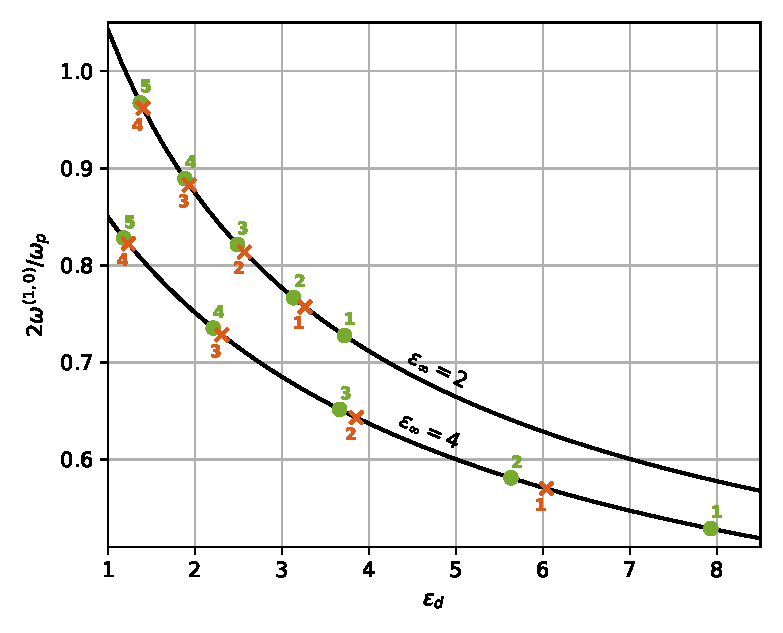
\includegraphics[width=80mm]{./image/fig_w.eps}
	\caption{Положение частоты основного дипольного поверхностного резонанса (сплошная линия) в зависимости от диэлектрической проницаемости внешней среды, а также положения резонансных частот при $m=0,2$ (монопольные и квадрупольные объемные резонансы), при разной диэлектрической проницаемости ионного остова}
	\label{fig_w}
\end{figure} 
\newpage
\begin{figure}[h]
	\centering
	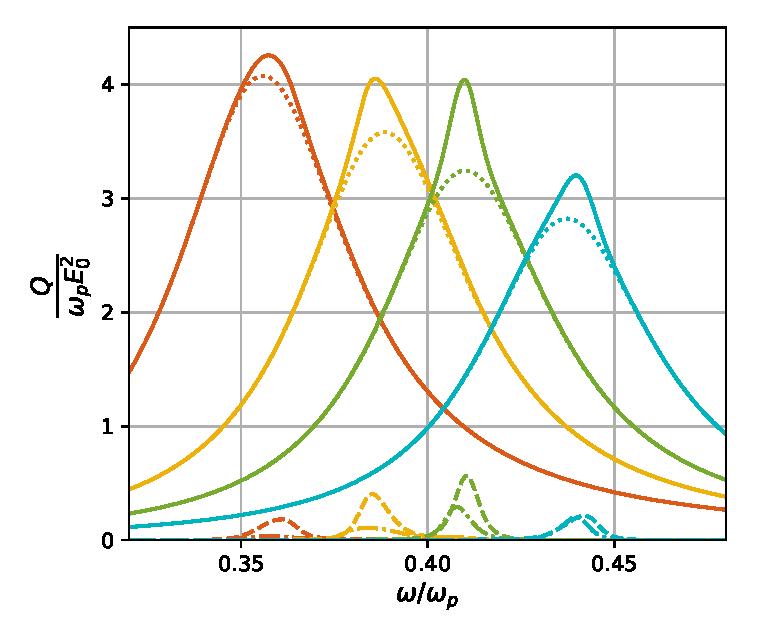
\includegraphics[width=80mm]{./image/fig1_epsd2.eps}
	\caption{Зависимость мощности потерь от частоты при $\eps_\infty= 2$, $\eps_d = 4, 3, 2.5, 2$ соответственно слева направо. Сплошной линией указана полная мощность потерь, точечной линией – вклад в потери от дипольных колебаний, пунктир и пунктир с точкой вклад от монопольных и квадрупольных колебаний соответственно. }
	\label{fig1_epsd2}
\end{figure} 
\newpage
\begin{figure}[h]
	\centering
	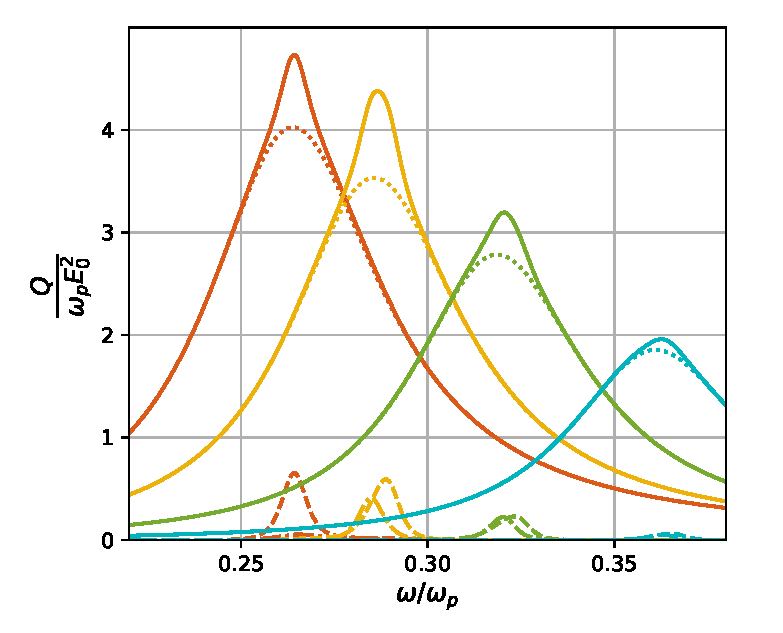
\includegraphics[width=80mm]{./image/fig1_epsd4.eps}
	\caption{Зависимость мощности потерь от частоты при $\eps_\infty= 4$, $\eps_d = 4, 3, 2.5, 2$ соответственно слева направо. Сплошной линией указана полная мощность потерь, точечной линией – вклад в потери от дипольных колебаний, пунктир и пунктир с точкой вклад от монопольных и квадрупольных колебаний соответственно. }
	\label{fig1_epsd4}
\end{figure} 
\newpage
\begin{figure}[h]
	\centering
	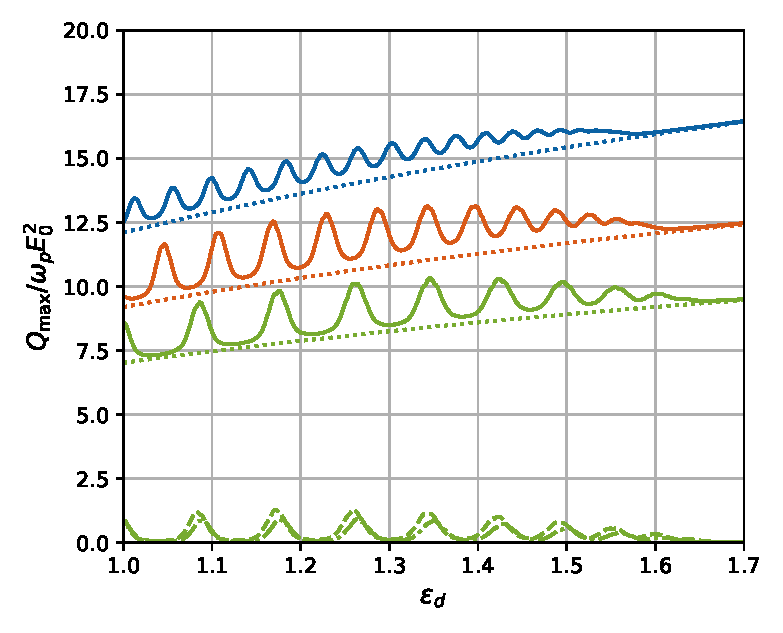
\includegraphics[width=80mm]{./image/natr2.eps}
	\caption{Зависимости максимальной мощности потерь для сферических наночастиц натрия радиусом 10 нм, 7 нм, 5 нм сверху вниз соответственно. Сплошной линией указана полная мощность потерь, точечной линией – вклад в потери от дипольных колебаний. В нижней части графика для наночастицы радиусом 5 нм пунктиром и пунктиром с точкой показан вклад от монопольных и квадрупольных колебаний соответственно.}
	\label{natr}
\end{figure} 
\end{document}
